%!TEX root = ../presentation.tex
\section{Live Demo}

\section{Fragen?}

\begin{frame}{}
    \thispagestyle{plain}
\end{frame}

\begin{frame}{Kalenderansicht im Darkmode}
    \thispagestyle{plain}
    \begin{figure}
        \centering
        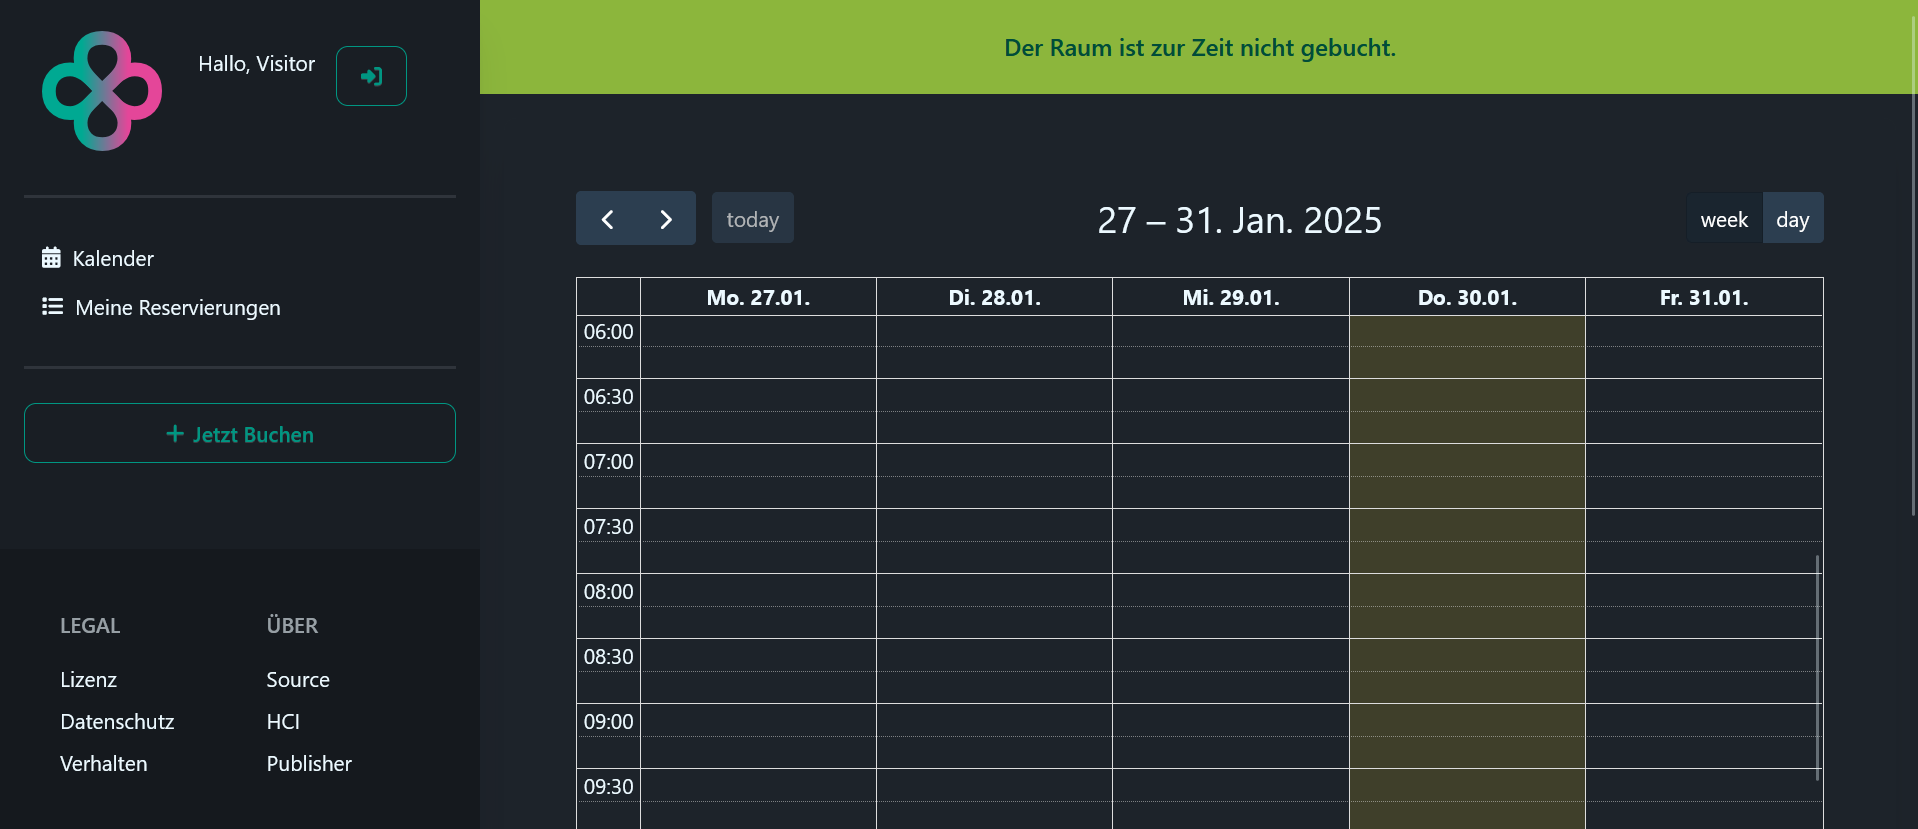
\includegraphics[width=1\linewidth]{pictures/calendar_dark.png}
        \label{fig:enter-label}
    \end{figure}
\end{frame}

\begin{frame}{Termin erstellen}
    \thispagestyle{plain}
    \begin{figure}
        \centering
        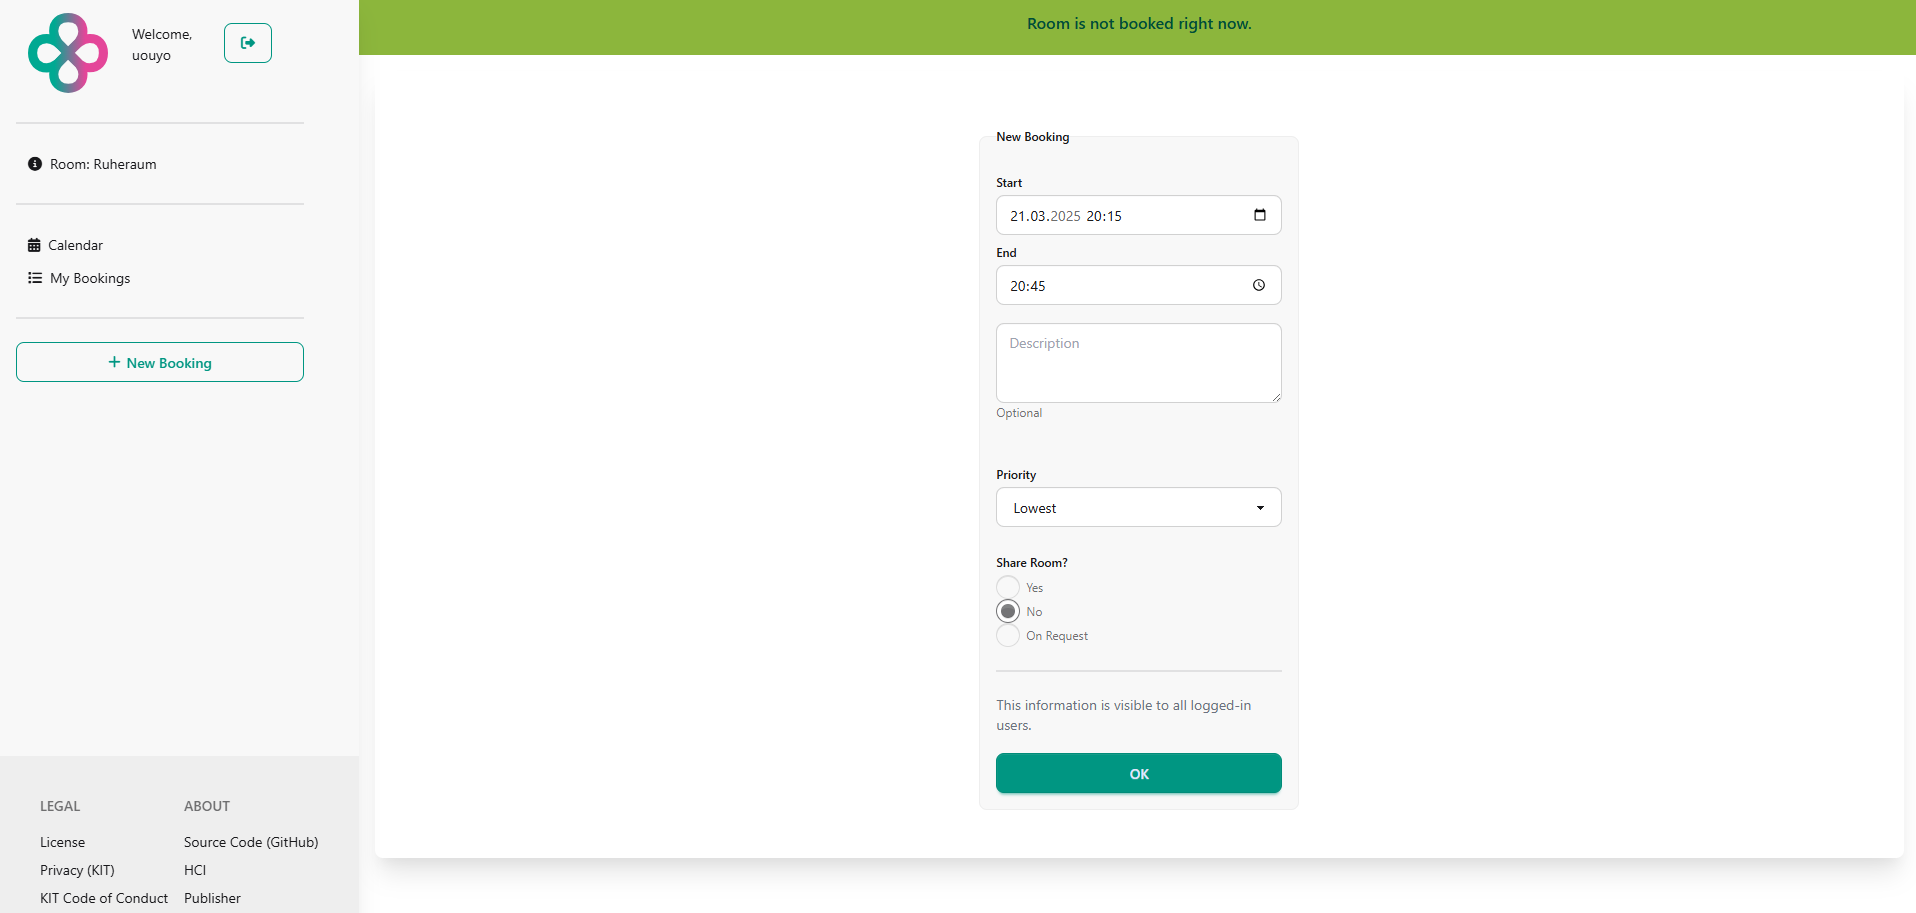
\includegraphics[width=1\linewidth]{pictures/bookings_create.png}
        \label{fig:enter-label}
    \end{figure}
\end{frame}

\begin{frame}{Konfliktauflösung}
    \thispagestyle{plain}
    \begin{figure}
        \centering
        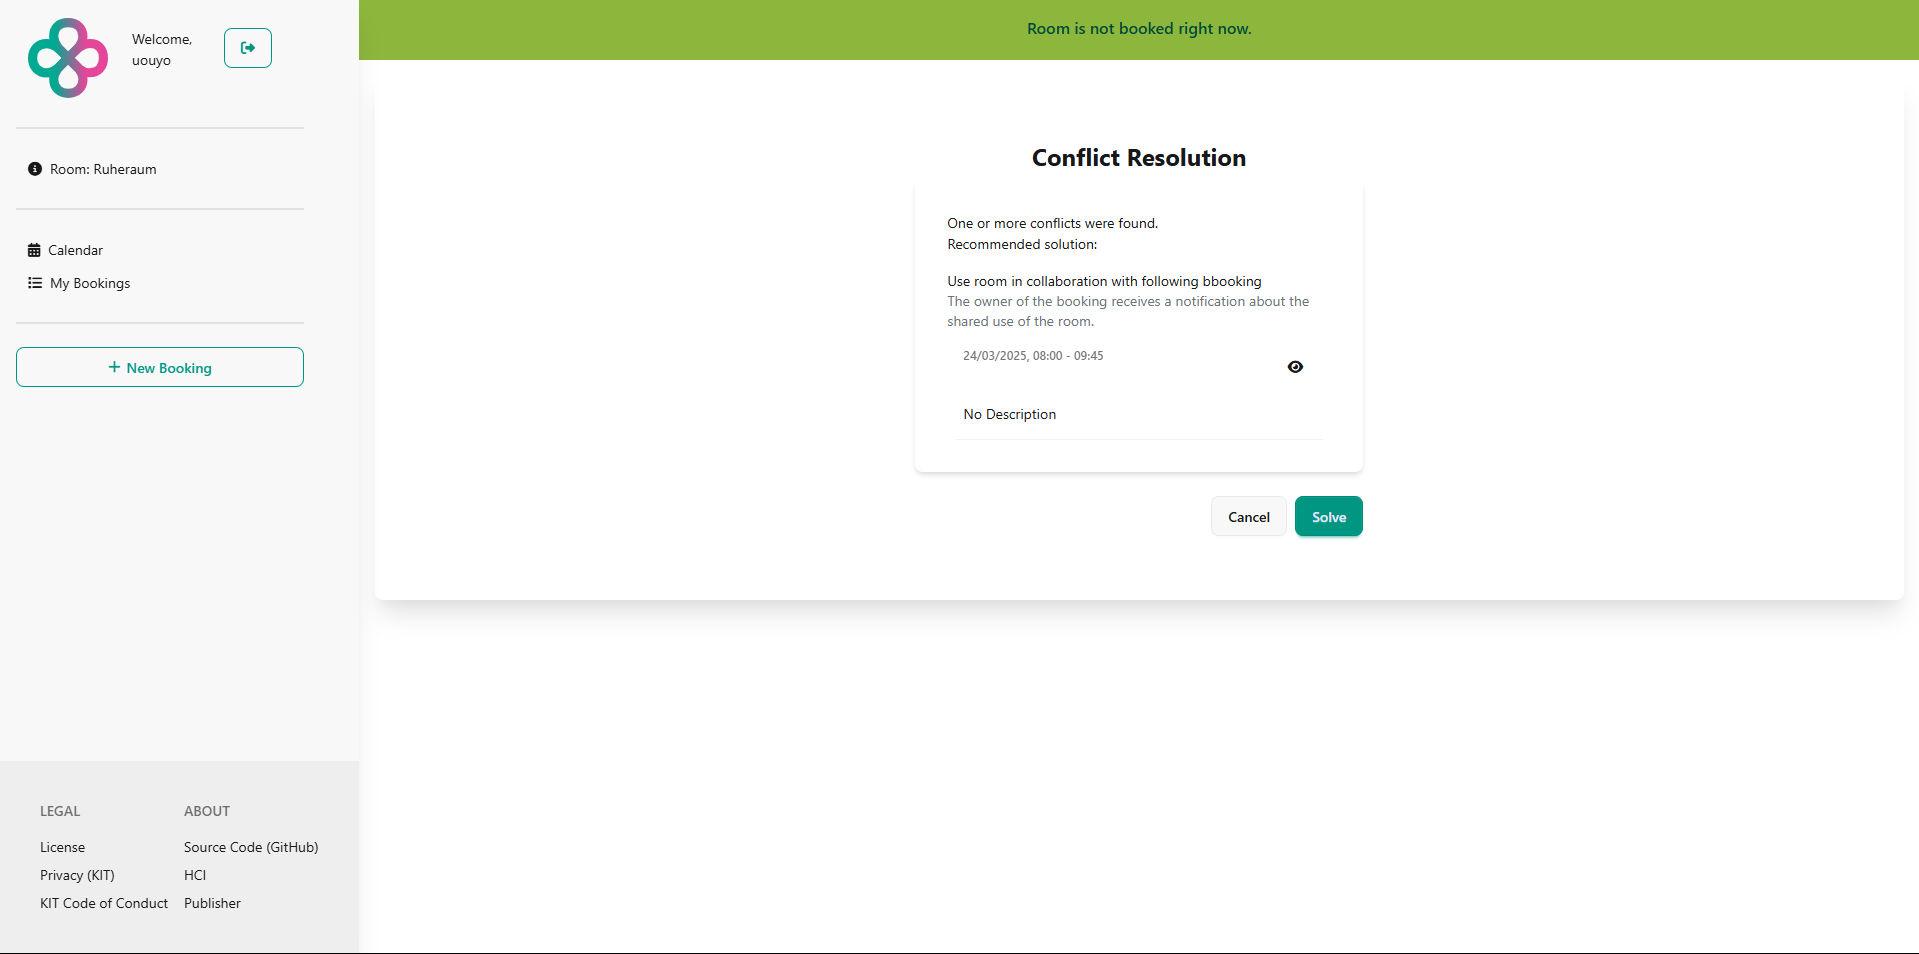
\includegraphics[width=1\linewidth]{pictures/conflict_resolution.png}
        
        \label{fig:enter-label}
    \end{figure}
\end{frame}

\begin{frame}{Anmeldeseite}
    \thispagestyle{plain}
    \begin{figure}
        \centering
        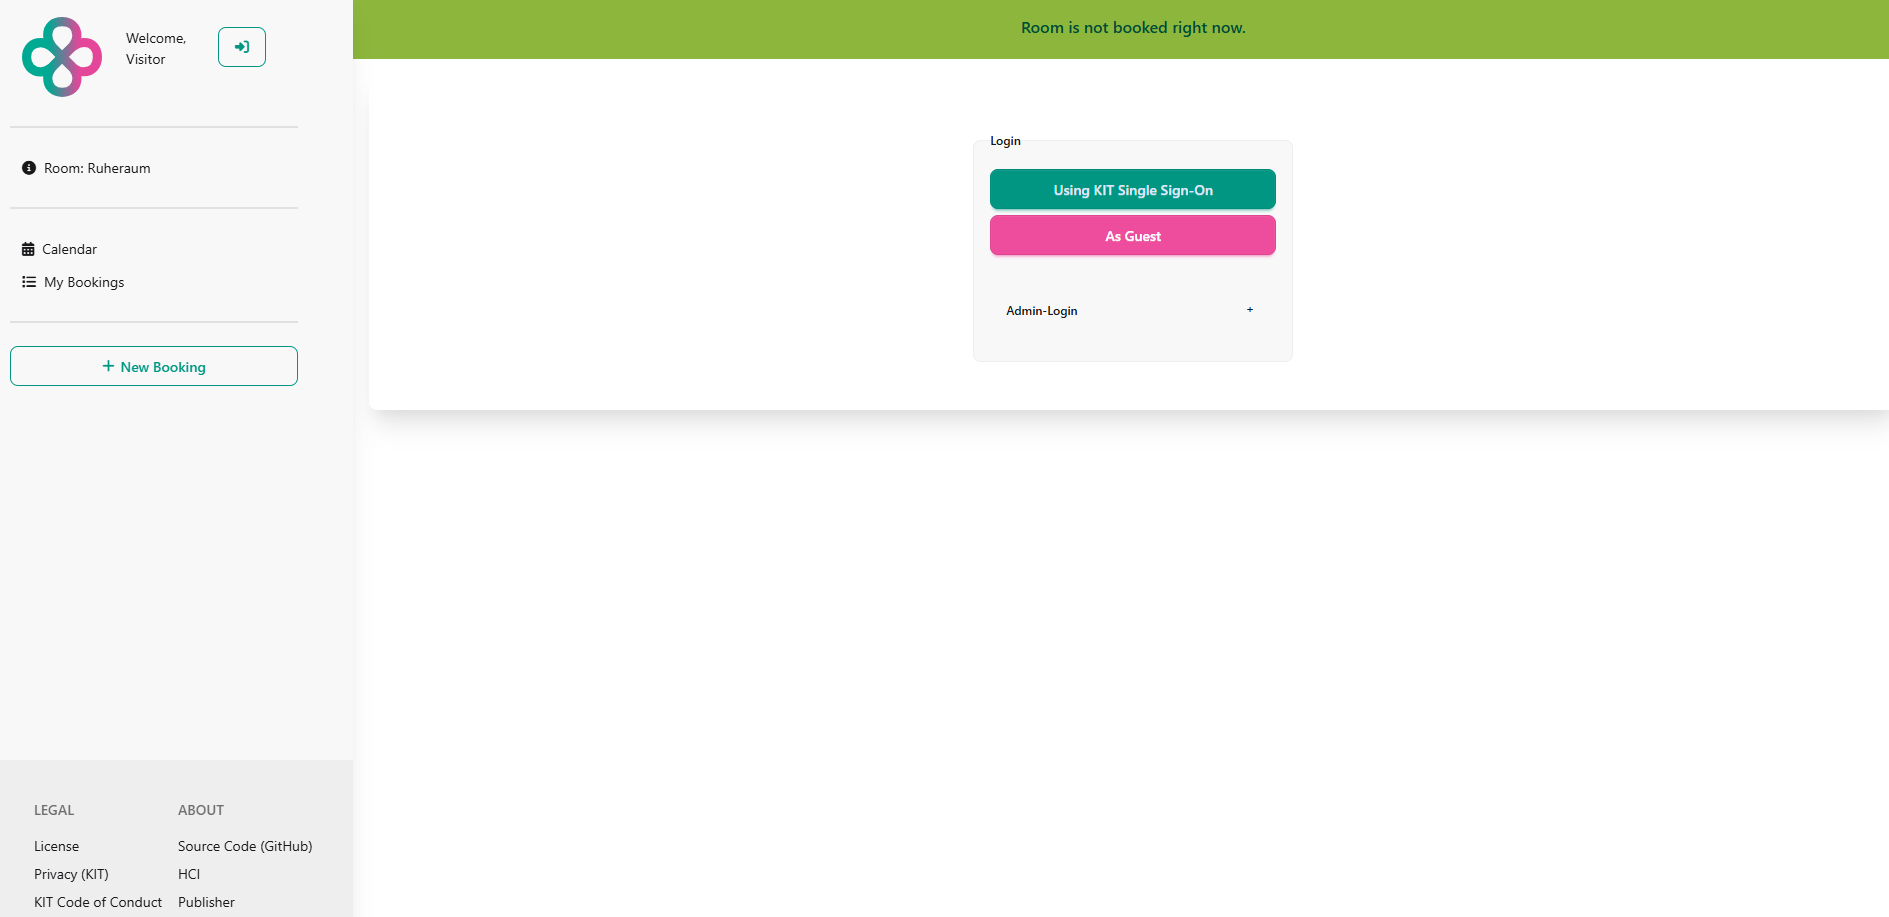
\includegraphics[width=1\linewidth]{pictures/auth_login.png}
        \caption{Login}
        \label{fig:enter-label}
    \end{figure}
\end{frame}

\begin{frame}{Reservierungsübersicht}
    \thispagestyle{plain}
    \begin{figure}
        \centering
        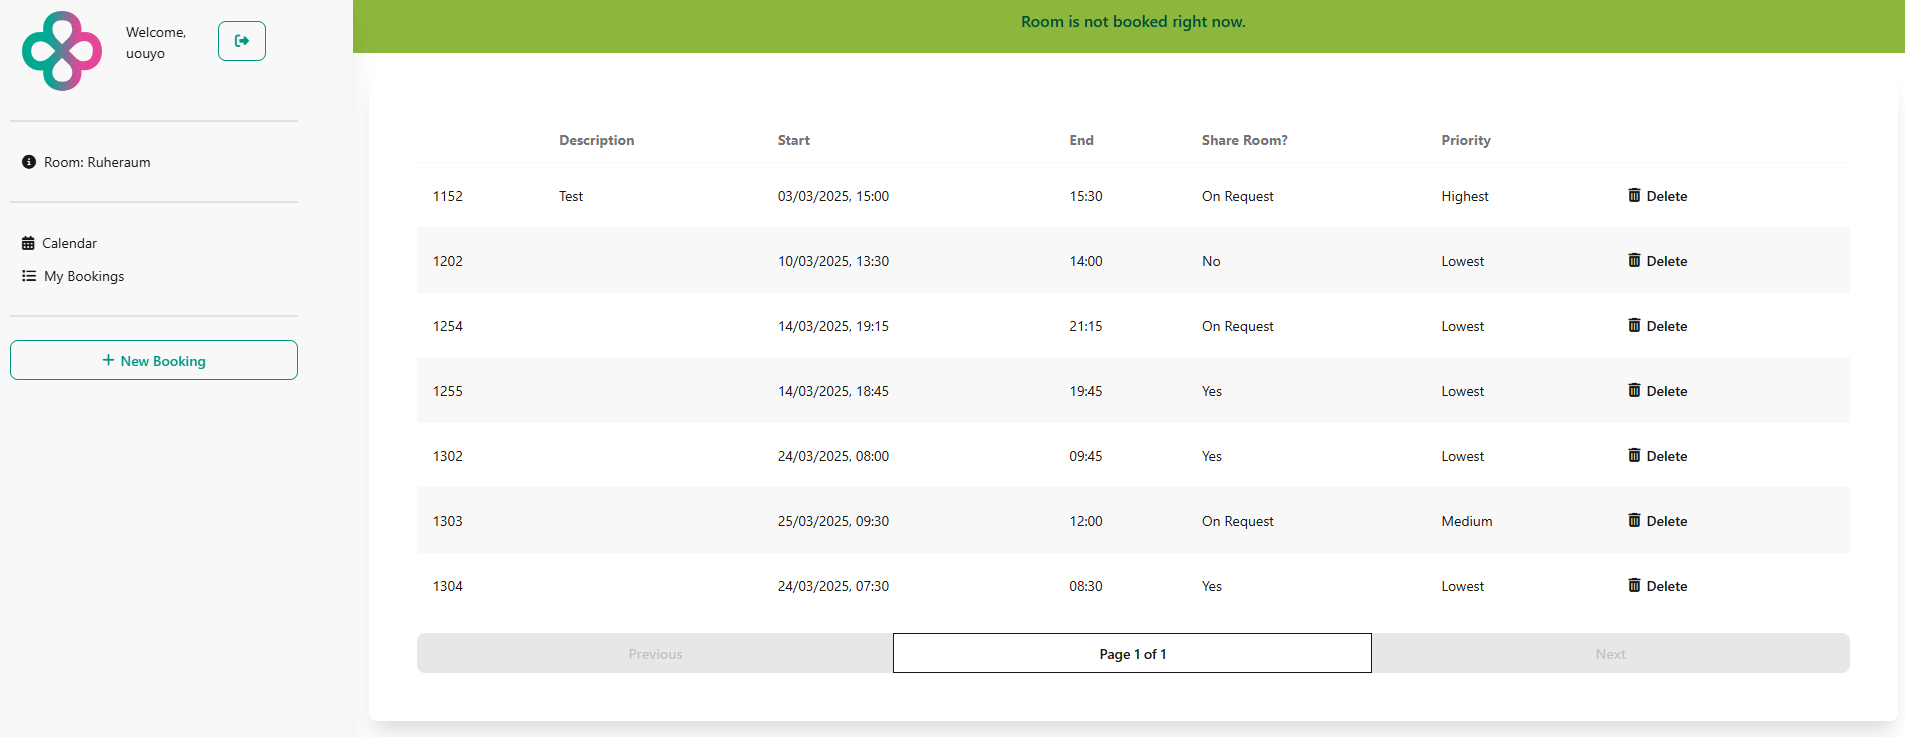
\includegraphics[width=1\linewidth]{pictures/bookings_list.png}
        \label{fig:enter-label}
    \end{figure}
\end{frame}

\begin{frame}{Reservierung im Kalender}
    \thispagestyle{plain}
    \begin{figure}
        \centering
        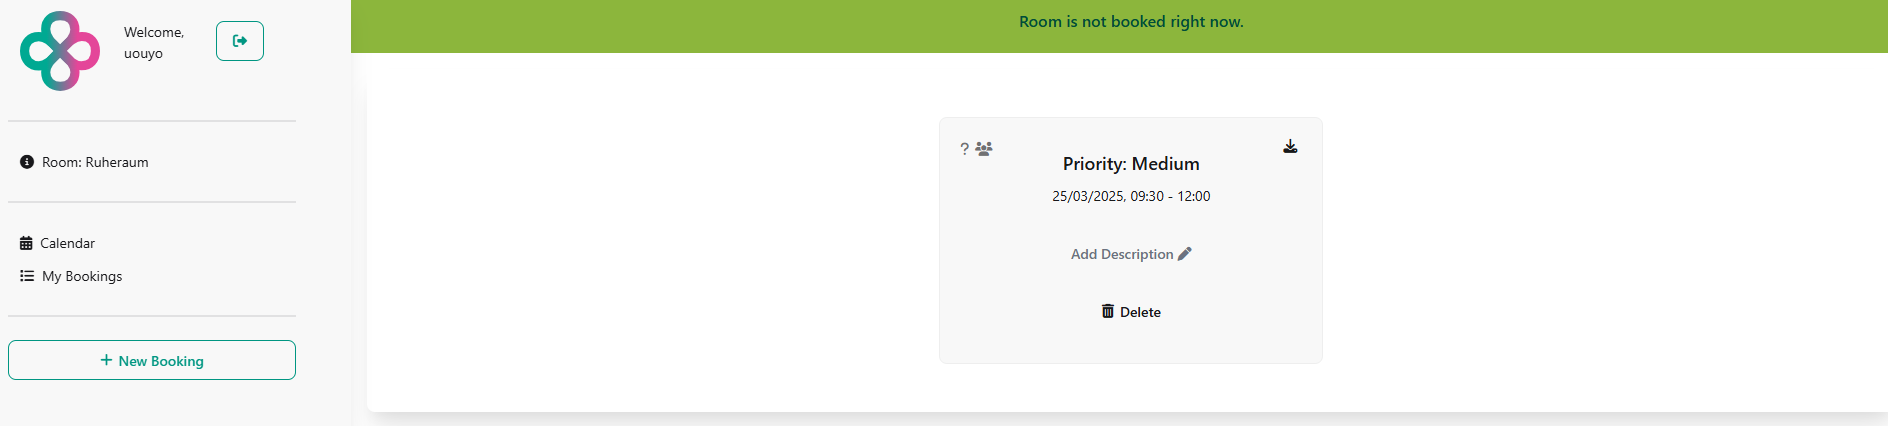
\includegraphics[width=1\linewidth]{pictures/bookings_single.png}
        \label{fig:enter-label}
    \end{figure}
\end{frame}

\begin{frame}{Quick Checkout Button}
    \thispagestyle{plain}
    \begin{figure}
        \centering
        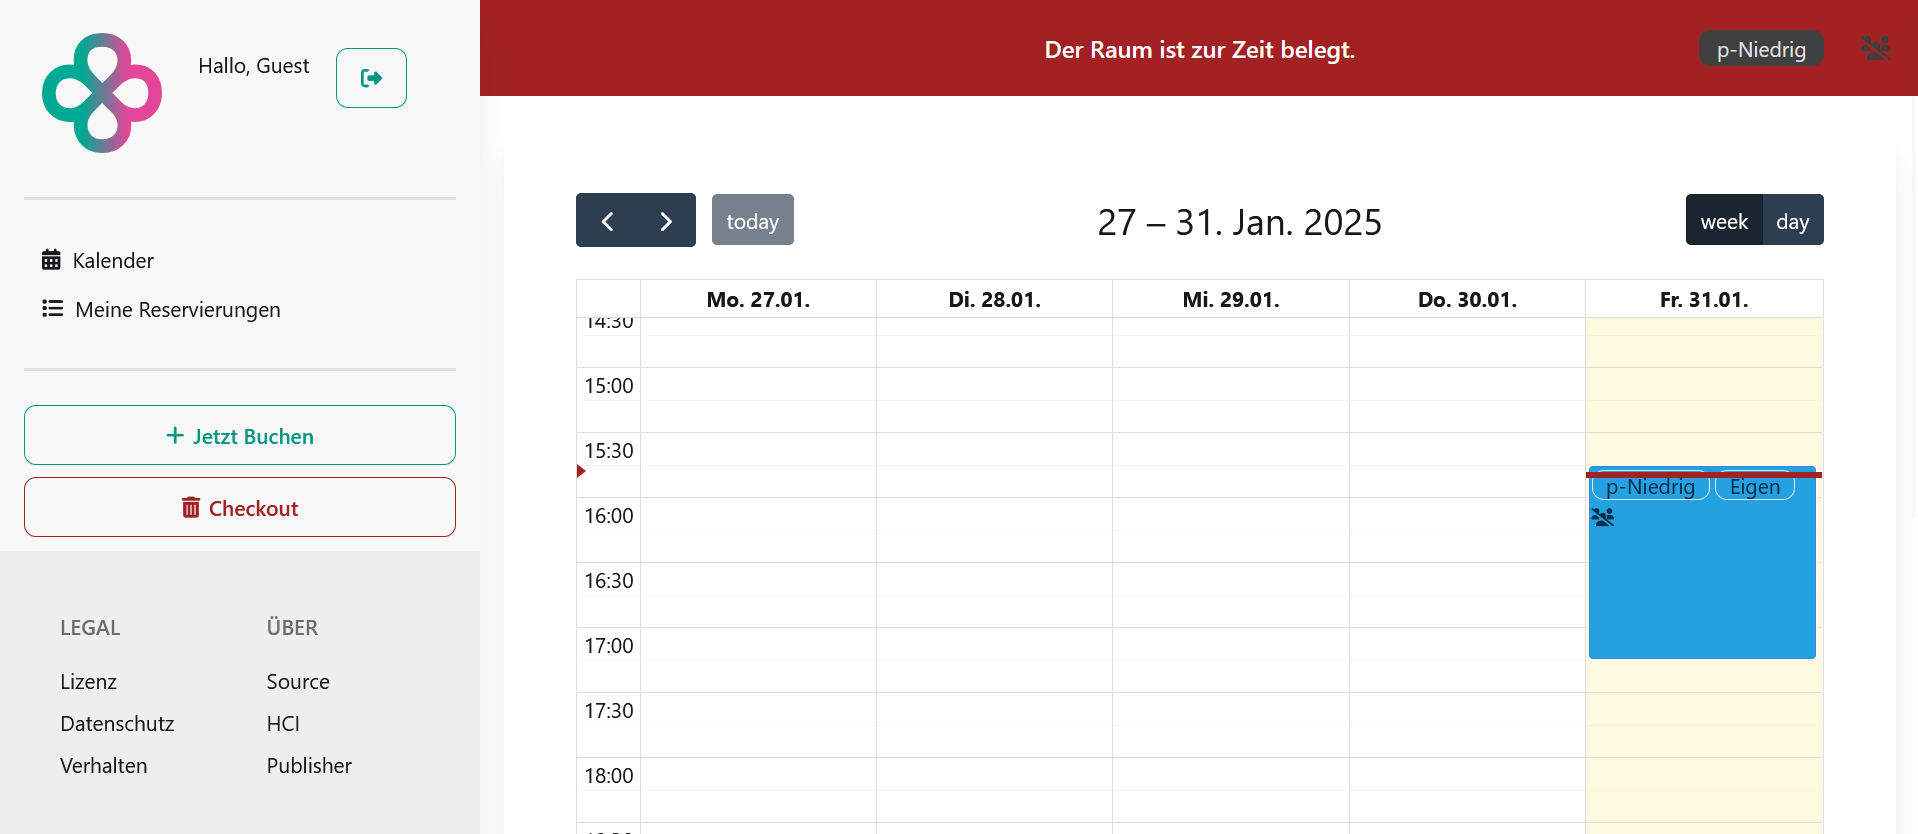
\includegraphics[width=1\linewidth]{pictures/check_out_button_light.png}
        \label{fig:enter-label}
    \end{figure}
\end{frame}
